\documentclass[11pt,twoside]{report}
\usepackage{mathptmx}
\renewcommand{\baselinestretch}{1.2}
\usepackage[english]{babel}
\usepackage{biblatex}
\usepackage{listing}
\usepackage{lscape}
\addbibresource{Bachelor's Thesis.bib}
\usepackage[utf8]{inputenc}
\usepackage{graphicx}
\usepackage[a4paper,top=20mm,bottom=20mm,right=20mm,left=33mm]{geometry}
\usepackage{fancyhdr}
\usepackage{csquotes}
\usepackage{float}
\pagestyle{fancy}
\fancyhead{}
\fancyhead[RO,LE]{Geolocalization and routing in complex multi-floor hospital environments}
\fancyfoot{}
\fancyfoot[LE,RO]{\thepage}
\fancyfoot[LO,CE]{Chapter \thechapter}
\fancyfoot[CO,RE]{Joachim Cardoen}
\renewcommand{\headrulewidth}{0.4pt}
\renewcommand{\footrulewidth}{0.4pt}
\usepackage[acronym]{glossaries}
\makeglossaries
\newglossaryentry{latex}
{
    name=latex,
    description={Is a mark up language specially suited 
    for scientific documents}
}
 
\newglossaryentry{maths}
{
    name=mathematics,
    description={Mathematics is what mathematicians do}
}
\newacronym{poc}{PoC}{proof of concept}
\newacronym{pwa}{PWA}{progressive web application}
\newacronym{mvvm}{MVVM}{model-view-viewmodel}
\newacronym{ide}{IDE}{integrated development environment}
\newacronym{ux}{UX}{user experience}
\newacronym{api}{API}{application programming interface}
\newacronym{sdk}{SDK}{software development kit}
\newacronym{uml}{UML}{unified modelling language}
\newacronym{eu}{EU}{European Union}
\newacronym{dao}{DAO}{database access object}
\newacronym{ui}{UI}{user interface}
\title{
    {\large Bachelor's Thesis}\\
    {Geolocalization and routing in complex multi-floor hospital environments}\\
    {\large UC Odisee}\\
    {\large Department of Engineering Technology - Electronics and Information Technology, Specialisation Information Technology}
}
\author{Joachim Cardoen}
\date{2018}
\graphicspath{{figures/}}
\setlength\headheight{15pt}

\begin{document}
\begin{titlepage}
\maketitle
\end{titlepage}
\begin{center}
I want to thank my foster mother, Miek Roels for her devotion to guide me through the process of writing this thesis. I want to thank her and both Nathan Verhoeven, one of my closest friends, as well as Cedric De Roover (Senior Consultant Manager at IBM) to correct my thesis where necessary. I also want to thank my mentor Sven Sanders for answering my e-mails day and night whenever I had got stuck.
\end{center}
\chapter*{Abstract}
The aim of this project is to realize a mobile application for patients of the hospital CHC Saint-Jean in Liege that will enable them to register,
view appointments and find their way in the hospital.
First the existing application for consulting scheduled appointments and registration is reworked to a native iOS mobile application (mobile app in short).
This feature is extended with the option to view the information of the hospital and set reminders for any appointment in the near future.
Second an indoor location framework is added to the reworked mobile app that shows the route to the place of appointment.
After implementing the geolocation and routing, an optimization method is implemented: the ant colony optimization algorithm.
The ant colony algorithm determines the shortest path to the place of appointment based on some factors such are: amount of visitors in some corridors and hallways and
the amount of stairs a patient has to climb (a patient's mobility). Using the mobile app the hospital can improve their safety procedures by notifying users of the
application of any problems in the hospital, these problems can be but are not limited to: fire, malfunctioning of the elevator and electrical outage.
\tableofcontents
\clearpage
\printglossary[type=\acronymtype]
\printglossary
\chapter{Summary}
\chapter{Project Specification}
\section{Project Description}
This bachelor's thesis covers a case study provided by IBM, related to an internship performed at IBM. This chapter will cover the case study, specific requirements and which technologies need to be researched and thus are handled in this paper.
\subsection{Case Study}
\subparagraph{Applied case: patient location-based services in a hospital}
A hospital is a good example of why an \acrshort{ips} can be useful. Many people spend time following the indicated route from the hospital's hall to the specific point of interest (operation room, intensive care, specific doctor's office etc.), however this requires a patient or visitor to constantly check his current location and is therefore intolerant for human mistakes. The routing inside a hospital is a prime example of a static route which is not adaptive to the visitor and does not offer real-time changes. This is where the application of an \acrshort{ips} can be a dynamic technology to guide the user inside the building. Another important note is the user's privacy: when using the \acrshort{pn} location-based services it ensures the loss of connectivity - and thus the tracking of the user - when he or she is not in range of the positioning technology.
\subsection{Technologies to research}
Throughout the development of the PoC, several technologies are used, such are: Android \acrshort{sdk}, authentication, RoomDB for offline storage, IBM BlueMix \acrshort{api}, \acrfull{uml}, dependency injection, MapWize, IndoorLocation and Cisco CMX.
\chapter{Technical Study}
\section{Integrated Development Environment}
The application is written using Android Studio. Android Studio is an \acrshort{ide} supported by Google and based on the IntelliJ \acrshort{ide} of JetBrains, a company that develops an \acrshort{ide} for the most popular general purpose programming languages \cite{AndroidDevelopers2019c}.
\section{General Data Protection Regulation}
The General Data Protection Regulation of the \acrfull{eu} is a measure against possible theft of personal data and the protection of privacy, incorporated by the \acrshort{eu} and its member states in 2016. The general changes regarding the privacy directive of the \acrshort{eu} - firstly declared in 1995 - are as follows \cite{THEEUROPEANPARLIAMENTANDTHECOUNCILOF1995} \cite{EUGDPRPortal:byTrunomi2019}:
\begin{itemize}
\item Test
\end{itemize}

The application that is developed needs to take this specific regulation into account when it handles the personal data of a patient and the employees of the hospital. 
\section{Android Architecture}
\subsection{Testing}
\subsubsection{Testing Workflow}
70-20-10 rule
Red-green bar mantra is used by Google as the main testing workflow. First a failing test is written, then the code to pass the test is developed. After this process needed refactors are applied to the codebase.
\begin{figure}
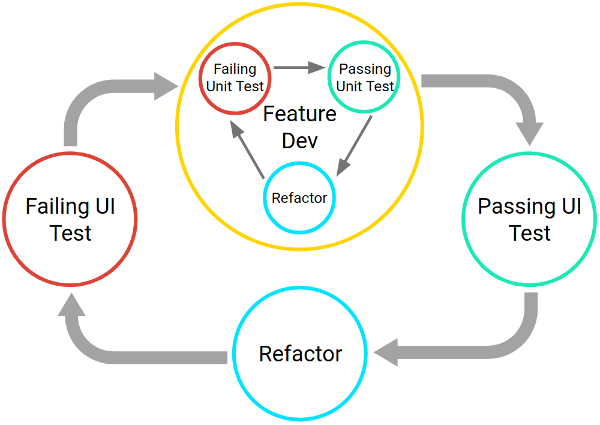
\includegraphics[scale=0.5]{testing-workflow}
\centering
\caption{Testing workflow~\cite{Google_testing2017}}
\end{figure}
\begin{figure}[h!]
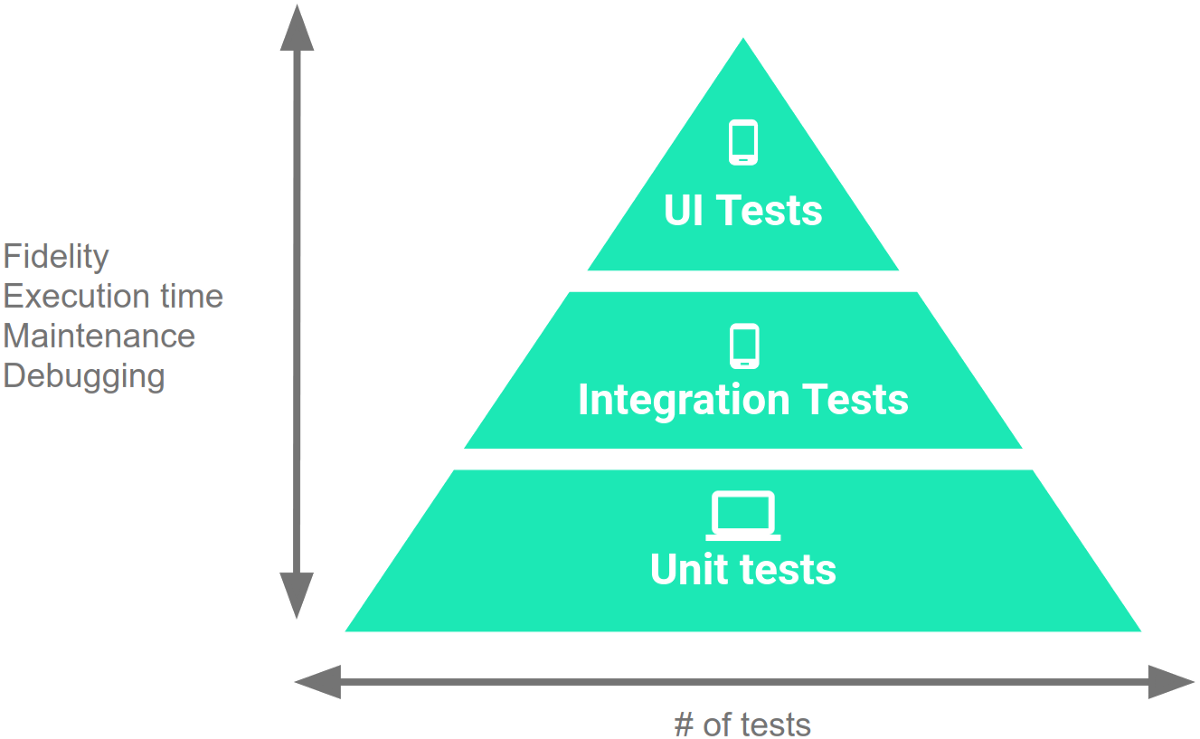
\includegraphics[scale=0.25]{testing_android}
\centering
\caption{Testing pyramid~\cite{FernandoSproviero2018}}
\end{figure}
\subsubsection{Unit Testing}
These tests are responsible for the smaller parts of the application (units) and use mocked or stubbed properties. This means that the properties and methods do not interfere with code written inside the main application. These tests are the fastest in runtime (compared to the integration and UI testing) because they do not need a running device or emulator, which means they are the least expensive to execute. Some testing frameworks from Android are: JUnit4 and Mockito (Mockito is used to create mock instances of dependencies, classes, properties and methods) \cite{FernandoSproviero2018}. The characteristics of a good unit test are \cite{Google_testing2017}:
\begin{enumerate}
\item Thorough;
\item Focused;
\item Repeatable;
\item Fast;
\item Verifies behaviour;
\item Concise;
\end{enumerate}
\subsubsection{Integration Testing}
These tests test the interaction between different units of the application. The tests do not cover any updates on the UI thread and test the units independently from the UI. A common framework used to write integration tests is Roboelectric \cite{Roboelec2019}. When an application is in development the integration tests will check the behaviour of the different interacting units when the new feature is implemented. This way, the development team can roll-out features without breaking the current application.
\subsubsection{User Interface Testing}
\subsection{Separation of concern: Dependency Injection}
Separation of concern is a general convention amongst software developers. In practice it is harder to implement than it first seems. One of the core components of this pattern are dependencies: one class depends on the structure of another class. The dependency pattern enables developers to focus on their code without having to worry about the dependency. For a class it is enough to know how a dependency is structure, there is no need for the class to know how it is implemented. This is also the last of the SOLID principles, the principle of dependency on abstraction instead of concrete implementation \cite{BhavyaKaria2018}.
\subsubsection{Dependency Injection: Restaurant Analogy}
To comprehend the concept of dependency injection let's have a look at a fairly common analogy". A man comes into a restaurant and takes a look at the menu. After having taken a close look, the man decides to order fish and chips. The waiter notifies the kitchen and tells the head chef that a customer ordered the fish and chips. Upon finishing the plating, the waiter brings the wonderful plate of fish and chips to the customer (the man). The man obtained what he wanted without knowing how his dish was prepared, the head chef knew what the customer needed and provided the meal.
\subsubsection{Benefits of using Dependency Injection}
Using dependency injection might seem somewhat bloated in practice, but there are some enormous benefits upon applying this pattern on an application. Some of these benefits are listed below \cite{Seemann2011}:
\begin{itemize}
\item Late binding: interchangeable services;
\item Extensibility: reusable code;
\item Maintainability: classes with a well-defined responsibility become easier to maintain;
\item Testability: classes having a dependency can be tested separately - as a single unit; 
\item Enforces usage of loose coupling;
\end{itemize}
\subsubsection{Types of Dependency Injection}
Constructor injection is the type of DI (dependency injection) that uses a private field for the dependency and sets this field using a parameter inside of the constructor. Setter (property) injection uses a property of the class that requires the dependency and works via getter and setter methods. The dependency is individually set instead of passed as a parameter in the constructor. This is quite easy to understand but hard to implement in a robust way, this only works if the value passed in the setter is a good value. When dependencies are only used in specific methods, it might be easier to just pass them as parameters to that method, this is called method injection. This way of implementing DI is also simple and straightforward \cite{TheoJungeblut2015}.
\subsection{Lifecycle Events}
For the duration of the runtime of the mobile application (from the moment the app is opened until it is closed) some events occur that are typical for an Android mobile application. A brief summary of these events is listed below (in chronological order) \cite{AndroidDeveloper2019}:
\begin{itemize}
\item onCreate() - When the activity is launched (This can happen after the onDestroy() event);
\item onStart() - When the activity is visible to the user;
\item onResume() - When the user returns to the activity after an onPause() event occurs;
\item onPause() - When activity is no longer visible;
\item onStop() - When the activity is finished or destroyed;
\item onRestart() - When the activity is restarted after a stoppage;
\item onDestroy() - When the activity is shut down;
\end{itemize}
\begin{figure}[H]
\centering
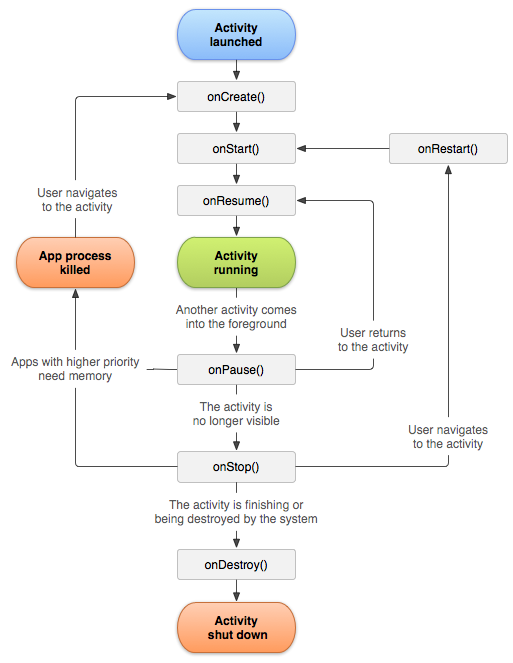
\includegraphics[scale=0.5]{activity_lifecycle}
\caption{Android Activity Lifecycle Schematic~\cite{AndroidDeveloper2019}}
\end{figure}
The lifecycle of an activity is an important factor to take into account whilst the application is being developed. This means a certain level of persistency is required for an optimal user experience.
\subsubsection{Bundles \& Saved State}
The way in which the onCreate() method is implemented allows a developer to declare a Bundle, which is an object that contains key-value pairs, that is used to restore an activity's previous state. If no such state exists then the Bundle will be equal to null. The Bundle object that is passed to an activity in the onCreate() method should only contain specific information such as user interactions: form fields, position on the screen and sometimes navigational properties. The main usage for this technology is when an activity gets paused or stopped, this means the OS (operating system) can freely destroy any activities \cite{JamesHalpern2012}.
\subsection{Offline storage and persisting data}
Another way to persist data throughout the lifecycle of an application is to use the (smart)phone's local storage. Each application can create a new local database using SQLite. SQLite is a transactional and file-based database (db), which means it is optimal for storing user-specific data. The fact that it is indeed a transactional db means that upon failure of an operation it will roll-back to the previous state and revert all existing, pending changes \cite{TutorialsPoint2019}.
\subsection{Repository Design Pattern}
A common pattern to use for handling database communication the repository pattern. This pattern acts as an abstraction layer on top of the data layer and the business layer and centralises the domain models. One of the common ways of integrating the pattern is creating a \acrfull{dao} that interacts with the database of the application and a repository that can pass data from and to the \acrshort{dao}. Using the pattern as an additional abstraction layer enables easier testing and enforces the single responsibility principle \cite{Per-ErikBergman2017} \cite{NahidulHasan2018}.
\subsubsection{RoomDB}
A nice feature from the Android SDK is a wrapper for SQLite inside the app: RoomDB. RoomDB is a feature set for SQLite statement and works using the repository pattern. The interaction between the application (view layer) and data layer happens using a repository which can be implemented locally (offline storage using the RoomDB wrapper) as well as remotely (remote API calls). The structure of the application is as follows:
\begin{figure}[h!]
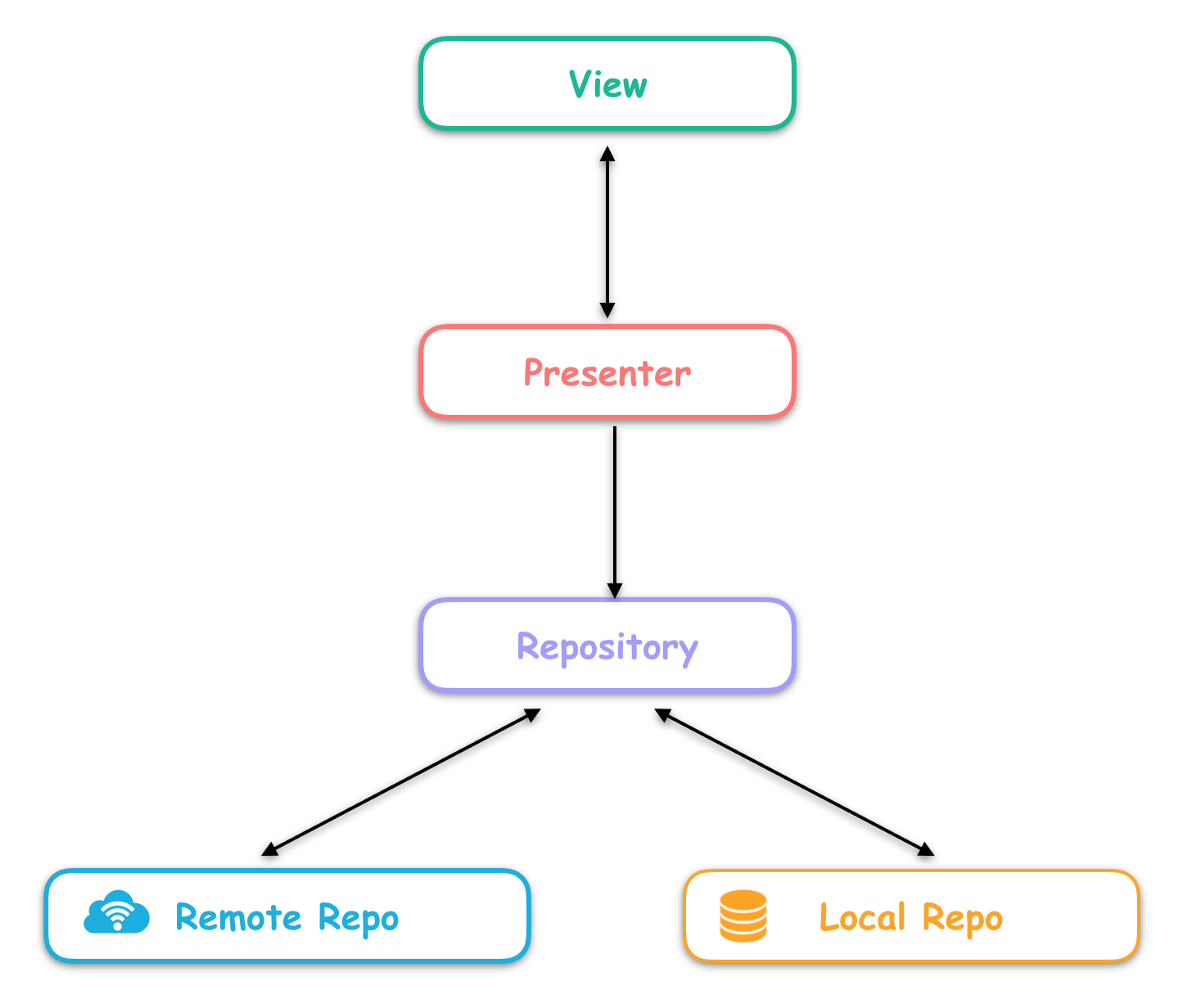
\includegraphics[scale=0.25]{repository_pattern_android}
\centering
\caption{Repository Pattern inside an android application~\cite{EslamHussein2018}}
\end{figure}
\begin{figure}[h!]
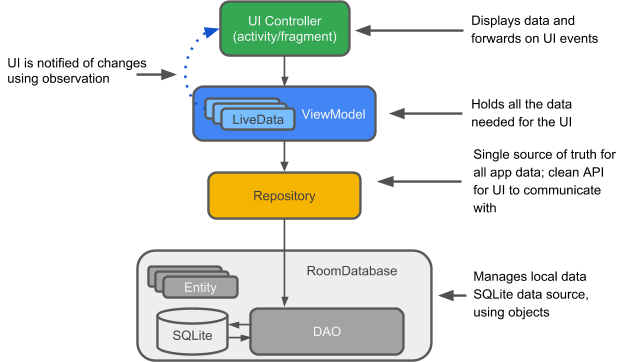
\includegraphics[scale=0.5]{local_repo_android}
\centering
\caption{Local repository usage inside the app~\cite{Unknown2018}}
\end{figure}
\subsection{Model - View - ViewModel Architecture}
One of the downsides of the default architecture of an Android application is the interaction between a view, model and layout files. Normally an activity is created with corresponding models which data needs to be presented in the view. This results in , possibly, a very large activity or fragment class. A good practice is to implement a Model-View-ViewModel architecture, which focuses on separating the different components required to generate a view, thus following the separation of concern principle. This principle is one that every developer should take into account, because it is the most important one. The prime advantage of using this principle is that is easier to maintain and opts for more testable components of your application \cite{AndroidDevelopers2019b}.
\subsubsection{UI Driven}
The optimal way of building an application is making the \acrshort{ui} dependent of a model, a class holding the data for a corresponding entity, preferably persistent. A model acts independently of an activity's or fragment's lifecycle and consequently independently of the concerns regarding handling lifecycles.
\subsubsection{Interaction between ViewModel - View}
An easy way of incorporating the viewmodel is via the ViewModelProvider class, which returns a reference to the ViewModel class specified. This viewmodel contains data that will drive the \acrshort{ui} and methods that will handle business logic. Typically the ViewModel has a LiveData list of the type of model that needs to be used and some references to a local and remote repository to fetch the data in an asynchronous fashion. The difficulty is to create a reactive \acrshort{ui}, that handles any changes to the data in the ViewModel object \cite{JaewoongEum2018}.
\subsubsection{LiveData and observables}
LiveData is a datatype that is lifecycle aware, meaning it will can monitor changes and notifies the \acrshort{ui} when that happens. The benefit of this datatype is the absence of any additional and rigid logic to handle the data binding. Methods returning LiveData can be observed using the observable pattern, the method is called from the ViewModel object and observed for changes in the LiveData that is returned by the method. This enables data-binding by only applying minor changes to the code inside the ViewModel and View \cite{AndroidDevelopers2019b}.
\begin{figure}[h!]
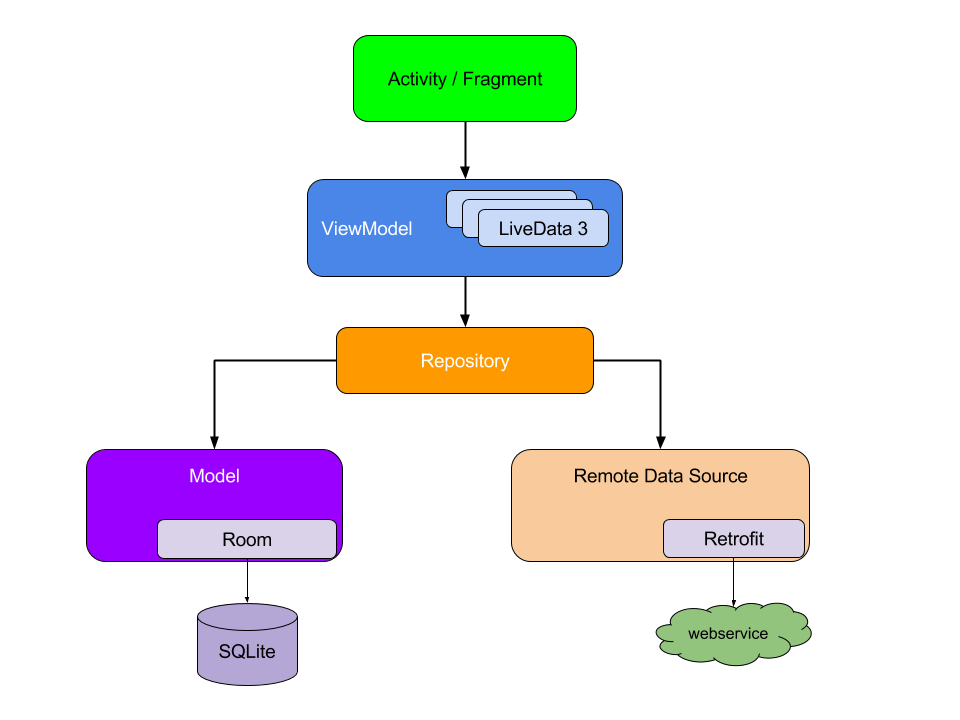
\includegraphics[scale=0.4]{app_architecture}
\centering
\caption{Complete architecture of application using ~\acrshort{mvvm}~\cite{AndroidDevelopers2019b}}
\end{figure}
\chapter{Proof of Concept}
\section{User Interface}
Considering the application is only a proof of concept (PoC) there is almost no focus on the user experience (UX) nor on the user interface (UI). To at least give a slight indication of what information needs to be displayed where, a UI mock-up is created in Adobe Xd, Adobe Xd is a lightweight, rudimentary visual editor that enables designers to quickly develop and share interactive prototypes. A few example screens of the UI prototype can be found below.
\begin{figure}[H]
\centering
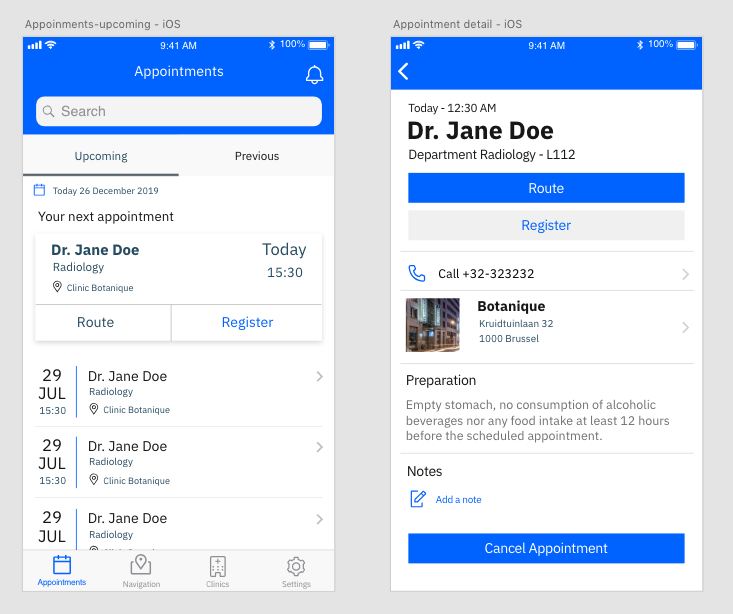
\includegraphics[scale=0.5]{appointments_screen_ios}
\caption{User interface of the appointments and detailed view for iOS}
\end{figure}
\begin{figure}[H]
\centering
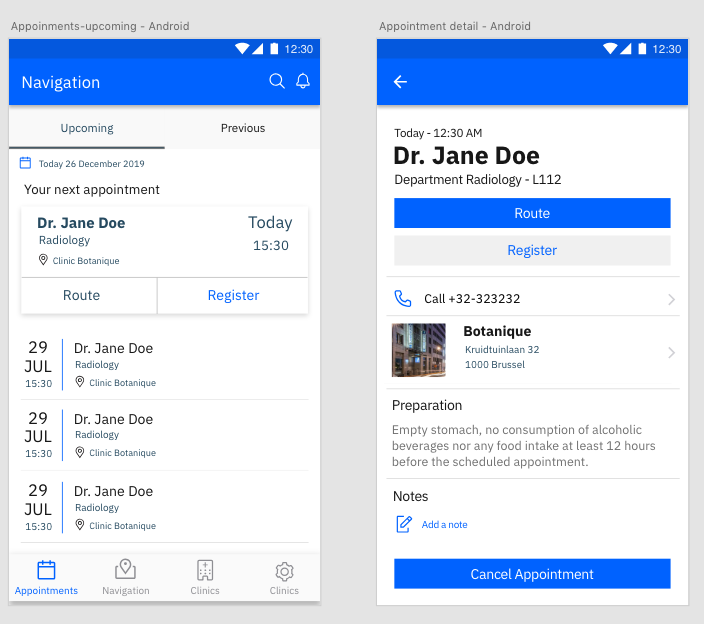
\includegraphics[scale=0.5]{appointments_screen_android}
\caption{User interface of the appointments and detailed view for Android}
\end{figure}
\begin{figure}[H]
\centering
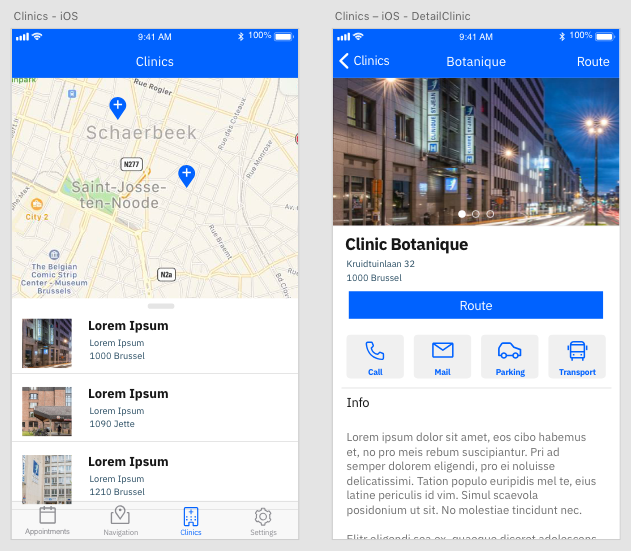
\includegraphics[scale=0.5]{clinics_screen_ios}
\caption{User interface of the hospital venues and detailed view for iOS}
\end{figure}
\begin{figure}[H]
\centering
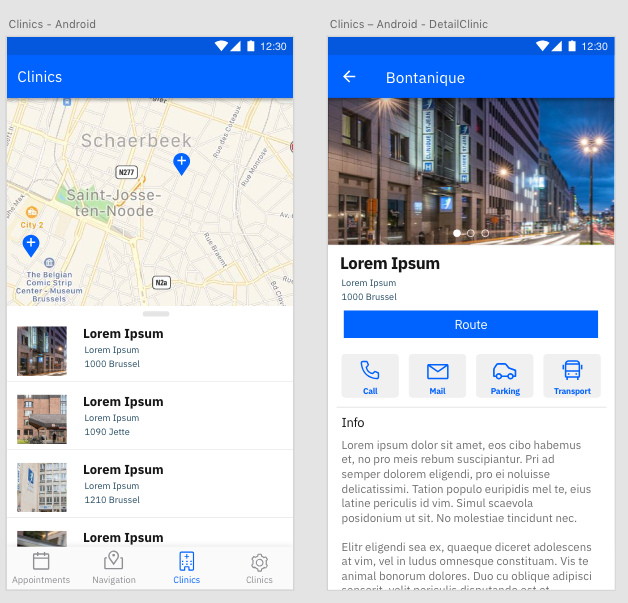
\includegraphics[scale=0.5]{clinics_screen_android}
\caption{User interface of the hospital venues and detailed view for Android}
\end{figure}
\section{General Data Protection Regulation}
\subsubsection{General Guidelines provided by the EU}
\section{Architecture}
The emphasis of the PoC is on developing it in such a way that it should be easy to re-implement the application elsewhere. The PoC is developed in the two current formats for mobile development: iOS and Android. This bachelor's thesis will cover the implementation of the Android architecture.
\subsection{Existing API}
The existing API developed by IBM provides the application with a list of appointments (testing mode). An example of the JSON output can be found below.
\subsubsection{Entities}
The specific entities used throughout this application are:
\begin{itemize}
\item appointment;
\item hospital;
\item venues - the different locations of a hospital;
\item address;
\item additionalinformation - meta for a hospital and venues;
\item department;
\end{itemize}
\subsubsection{UML Diagram}
\begin{landscape}
\begin{figure}[!h]
\centering
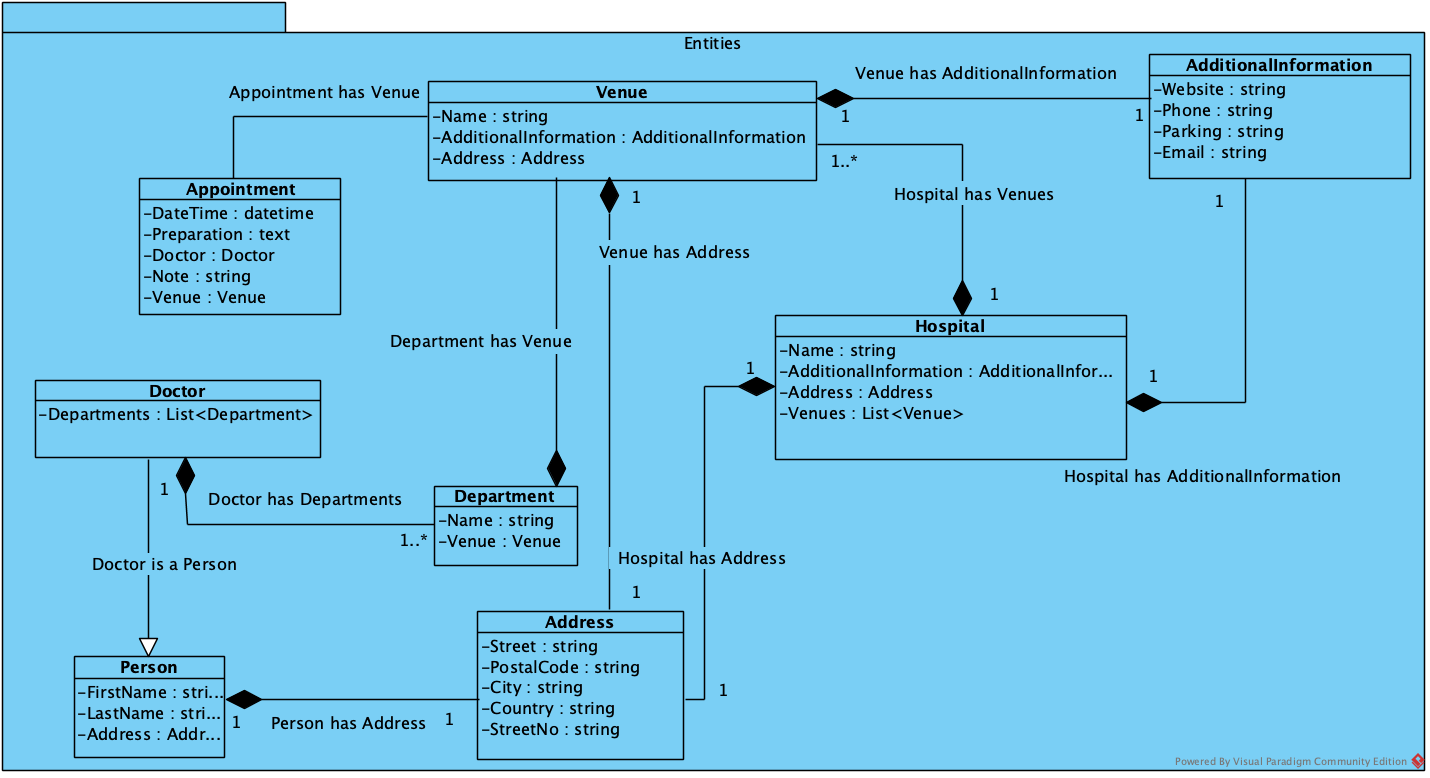
\includegraphics[scale=1]{UML_geolocalization}
\caption{Unified Modelling Language diagram}
\end{figure}
\end{landscape}
\section{Database Communication}
\subsection{Testing API}
To aid in testing the database a test API is programmed using a Node.js framework: Express. it is a very simple tool to create web APIs ready for consumption \cite{Express2019}. The testing API is structured according to the entities specified in the UML diagram with the corresponding relations. For this specific application there a couple of endpoints exposed for requests:
\begin{itemize}
\item GET /appointments - this returns a JSON array containing test appointments;
\item GET /hospital - this returns information about the hospital such as address, contact details and venues;
\item GET /doctors - this fetches all the doctors present in the hospital records;
\item GET /departments - this returns all the departments available in the hospital and its venues;
\end{itemize}
\subsubsection{Faker}
Instead of using ad random numerical combinations or lorem ipsum texts, a library called Faker is used to generate different random values such are names, addresses, e-mail addresses and phone numbers. Faker is available for almost every general purpose language and is easy to use. It is always easier to work with representative data than it is to work with 'lorem ipsum' or '123456789' \cite{DanieleFaraglia2014}.
\section{Android Architecture}
\subsection{Testing}
\cite{Google_testing2017}
\begin{figure}[h!]
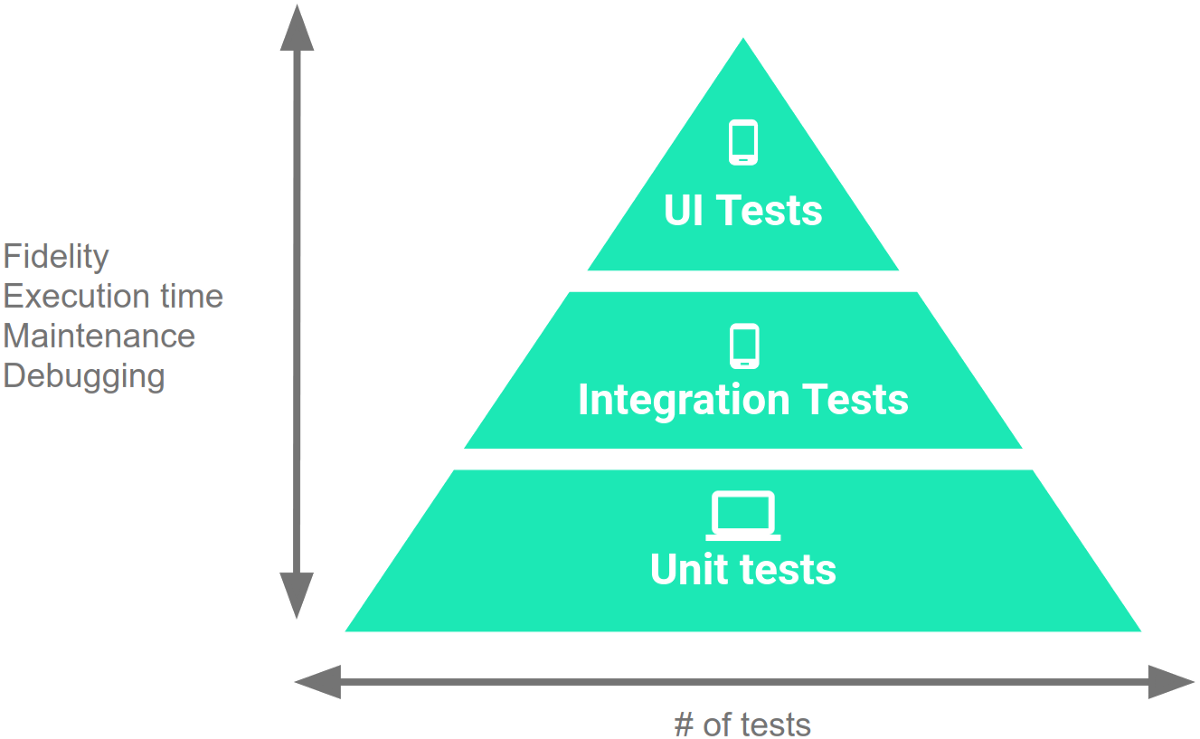
\includegraphics[scale=0.5]{testing_android}
\centering
\caption{Testing pyramid~\cite{FernandoSproviero2018}}
\end{figure}
\subsubsection{Unit Testing}
These tests are responsible for the smaller parts of the application (units) and use mocked or stubbed properties. This means that the properties and methods do not interfere with code written inside the main application. These tests are the fastest in runtime (compared to the integration and UI testing) because they do not need a running device or emulator, which means they are the least expensive to execute. Some testing frameworks from Android are: JUnit4 and Mockito (Mockito is used to create mock instances of dependencies, classes, properties and methods) \cite{FernandoSproviero2018}. The characteristics of a good unit test \cite{Google_testing2017}:
\begin{enumerate}
\item Thorough;
\item Focused;
\item Repeatable;
\item Fast;
\item Verifies behaviour;
\item Concise;
\end{enumerate}
\subsubsection{Integration Testing}
These tests test the interaction between different units of the application. The tests do not cover any updates on the UI thread and test the units independently from the UI. A common framework used to write integration tests is Roboelectric \cite{Roboelec2019}. When an application is in development the integration tests will check the behaviour of the different interacting units when the new feature is implemented. This way, the development team can roll-out features without breaking the current application.
\subsubsection{User Interface Testing}
\subsection{Separation of concern: Dependency Injection}
Separation of concern is a general convention amongst software developers. In practice it is harder to implement than it first seems. One of the core components of this pattern are dependencies: one class depends on the structure of another class. The dependency pattern enables developers to focus on their code without having to worry about the dependency. For a class it is enough to know how a dependency is structure, there is no need for the class to know how it is implemented. This is also the last of the SOLID principles, the principle of dependency on abstraction instead of concrete implementation \cite{BhavyaKaria2018}.
\subsubsection{Dependency Injection: Restaurant Analogy}
To comprehend the concept of dependency injection let's have a look at a fairly common analogy". A man comes into a restaurant and takes a look at the menu. After having taken a close look, the man decides to order fish and chips. The waiter notifies the kitchen and tells the head chef that a customer ordered the fish and chips. Upon finishing the plating, the waiter brings the wonderful plate of fish and chips to the customer (the man). The man obtained what he wanted without knowing how his dish was prepared, the head chef knew what the customer needed and provided the meal.
\subsubsection{Benefits of using Dependency Injection}
Using dependency injection might seem somewhat bloated in practice, but there are some enormous benefits upon applying this pattern on an application. Some of these benefits are listed below \cite{Seemann2011}:
\begin{itemize}
\item Late binding: interchangeable services;
\item Extensibility: reusable code;
\item Maintainability: classes with a well-defined responsibility become easier to maintain;
\item Testability: classes having a dependency can be tested separately - as a single unit; 
\item Enforces usage of loose coupling;
\end{itemize}
\subsubsection{Types of Dependency Injection}
Constructor injection is the type of DI (dependency injection) that uses a private field for the dependency and sets this field using a parameter inside of the constructor. Setter (property) injection uses a property of the class that requires the dependency and works via getter and setter methods. The dependency is individually set instead of passed as a parameter in the constructor. This is quite easy to understand but hard to implement in a robust way, this only works if the value passed in the setter is a good value. When dependencies are only used in specific methods, it might be easier to just pass them as parameters to that method, this is called method injection. This way of implementing DI is also simple and straightforward \cite{TheoJungeblut2015}.
\subsubsection{Dagger2 - Dependency Injection Library}
To remove the abstraction of the different methods of dependency injection, the library Dagger2 (supported by Google) is used. This library sets up the required dependencies throughout the application and registers them accordingly. Upon launching a class that requires a dependency, the Dagger2 instance will load them as specified in the AppModule.
\subsection{Kotlin Language}
\subsection{Lifecycle Events}
For the duration of the runtime of the mobile application (from the moment the app is opened until it is closed) some events occur that are typical for an Android mobile application. A brief summary of these events is listed below (in chronological order) \cite{AndroidDeveloper2019}:
\begin{itemize}
\item onCreate() - When the activity is launched (This can happen after the onDestroy() event);
\item onStart() - When the activity is visible to the user;
\item onResume() - When the user returns to the activity after an onPause() event occurs;
\item onPause() - When activity is no longer visible;
\item onStop() - When the activity is finished or destroyed;
\item onRestart() - When the activity is restarted after a stoppage;
\item onDestroy() - When the activity is shut down;
\end{itemize}
\begin{figure}[H]
\centering
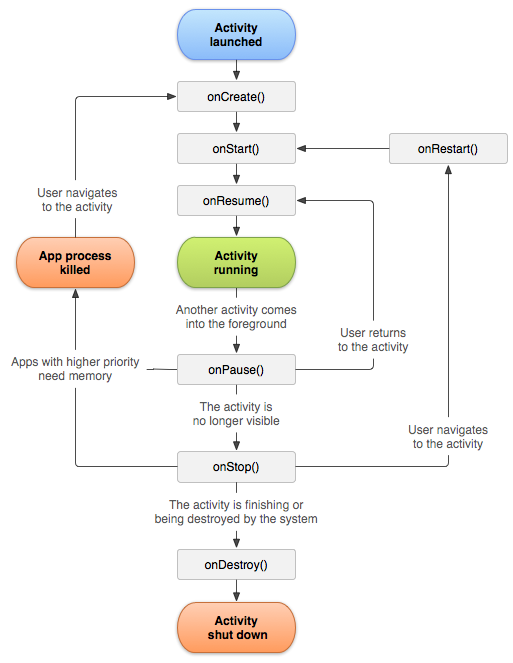
\includegraphics[scale=0.5]{activity_lifecycle}
\caption{Android Activity Lifecycle Schematic~\cite{AndroidDeveloper2019}}
\end{figure}
The lifecycle of an activity is an important factor to take into account whilst the application is being developed. This means a certain level of persistency is required for an optimal user experience.
\subsubsection{Bundles \& Saved State}
The way in which the onCreate() method is implemented allows a developer to declare a Bundle, which is an object that contains key-value pairs, that is used to restore an activity's previous state. If no such state exists then the Bundle will be equal to null. The Bundle object that is passed to an activity in the onCreate() method should only contain specific information such as user interactions: form fields, position on the screen and sometimes navigational properties. The main usage for this technology is when an activity gets paused or stopped, this means the OS (operating system) can freely destroy any activities \cite{JamesHalpern2012}.
\subsection{Offline storage and persisting data}
Another way to persist data throughout the lifecycle of an application is to use the (smart)phone's local storage. Each application can create a new local database using SQLite. SQLite is a transactional and file-based database (db), which means it is optimal for storing user-specific data. The fact that it is indeed a transactional db means that upon failure of an operation it will roll-back to the previous state and revert all existing, pending changes \cite{TutorialsPoint2019}.
\subsubsection{RoomDB}
A nice feature from the Android SDK is a wrapper for SQLite inside the app: RoomDB. RoomDB is a feature set for SQLite statement and works using the repository pattern. The interaction between the application (view layer) and data layer happens using a repository which can be implemented locally (offline storage using the RoomDB wrapper) as well as remotely (remote API calls). The structure of the application is as follows:
\begin{figure}[h!]
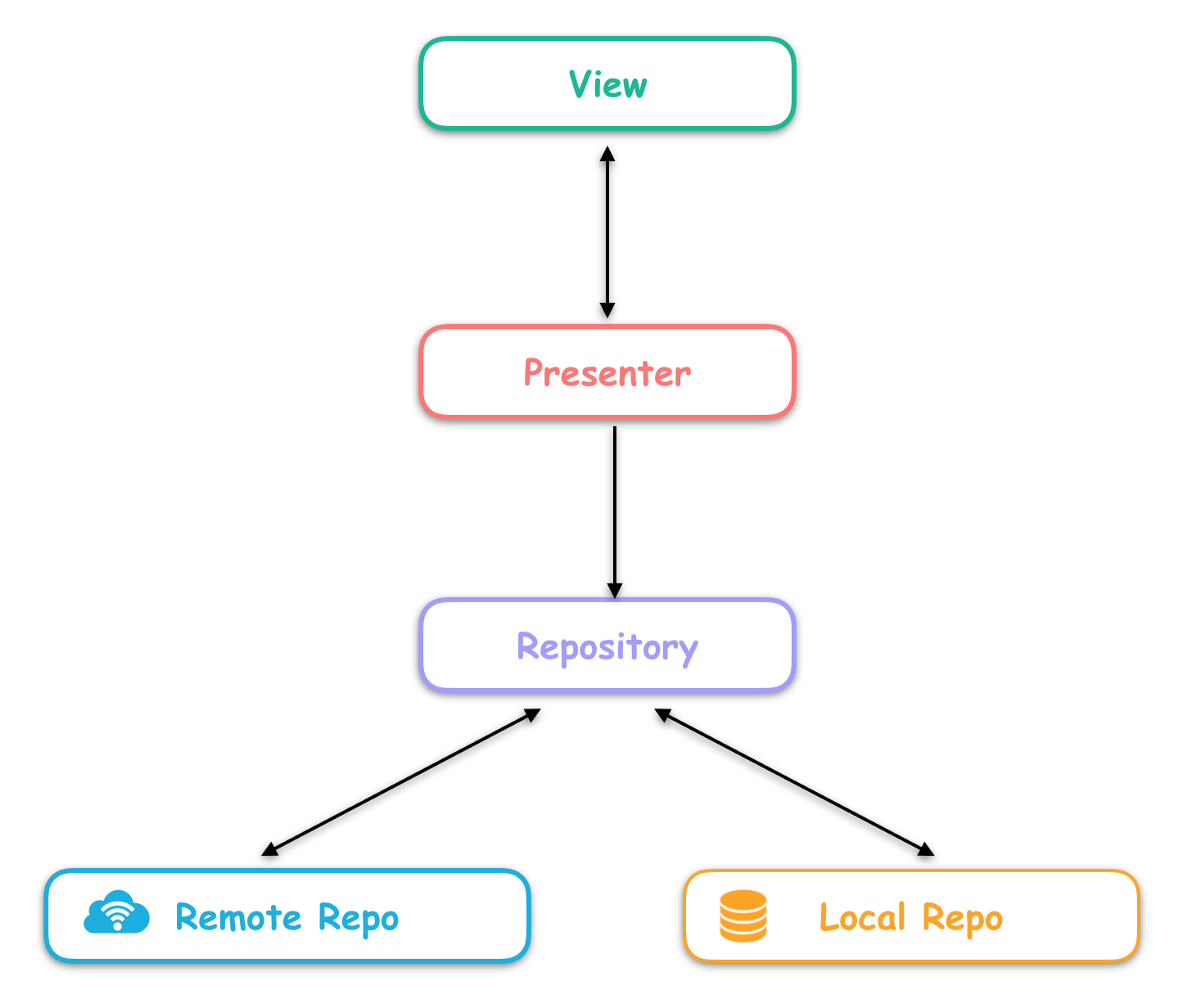
\includegraphics[scale=0.25]{repository_pattern_android}
\centering
\caption{Repository Pattern inside an android application~\cite{EslamHussein2018}}
\end{figure}
The local repository interacts with the local repository using a database access object, which specifies the different possible statements that can be executed on the database (CRUD operations: create, read, update and delete) and maps them to functions.
\begin{figure}[h!]
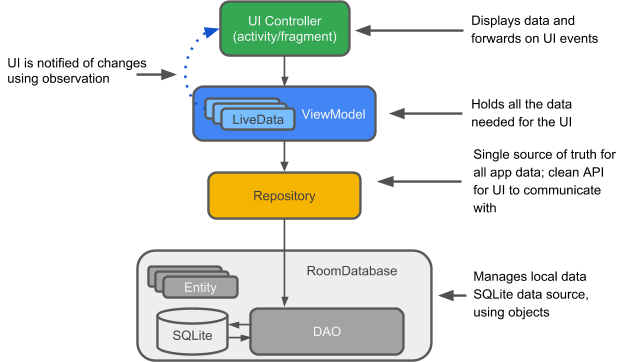
\includegraphics[scale=0.5]{local_repo_android}
\centering
\caption{Local repository usage inside the applocal~\cite{Unknown2018}}
\end{figure}

\subsubsection{Application Cache}
\subsubsection{Strategy and abstractions}
\subsection{Model - View - Presenter Architecture}
\subsubsection{Model}
\subsubsection{View}
\subsubsection{Presenter}
\subsection{Model - View - ViewModel Architecture}
\subsubsection{ViewModel}
\subsubsection{Asynchronous Data}
\subsubsection{HTTP(S) Requests}
\subsubsection{Retrofit}
\subsubsection{LiveData Datatype}
\subsubsection{Observables}
\section{Testing Application Programming Interface}
\section{Tools and frameworks used}
\section{MapWize}
MapWize is a service that digitalizes architectural plans and makes them interactive. MapWize offers an online environment in which you can easily create floor plans that can be used by the SDK. In the online editor you can declare specific points of interest (PoIs) and routes from and to points. The creation of a digital map for testing purposes is out of scope for this thesis. 

\subsection{MapWize SDK}
MapWize provides developers with a ready-made SDK for both iOS and Android. This SDK covers all important methods to 
\section{Cisco Connectected Mobile Experiences integration}
The manner in which the position of a patient is retrieved is based on the nearest WiFi router of Cisco.
\subsection{Function of Cisco CMX}
\section{IndoorLocation Framework}
The IndoorLocation framework is one heavily used in conjunction with MapWize, it is a framework that allows developer to use geolocalization based on numerous indoor positioning technologies (IPS) such are: GPS, beacons, Wi-Fi, Li-Fi, Ultrasounds etc \cite{IndoorLocation.io2019}.





\chapter{Conclusion}
\input{chapters/conclusion}

\appendix
\chapter{Development Guidelines}
\section{Source Code MapWize Activity}
\begin{lstlisting}
package com.ibm.geolocationframework.ViewLayer.Activities

class MapActivity : AppCompatActivity(), MapwizeFragment.OnFragmentInteractionListener {

    private var mapwizeFragment: MapwizeFragment? = null
    private var socketIndoorLocationProvider: SocketIndoorLocationProvider? = null
    private var mapwizePlugin: MapwizePlugin? = null
    private var mapboxMap: MapboxMap? = null

    override fun onCreate(savedInstanceState: Bundle?) {
        super.onCreate(savedInstanceState)
        setContentView(R.layout.activity_map)


        // Uncomment and fill place holder to test MapwizeUI on your venue
        val opts = MapOptions.Builder()
            .restrictContentToVenue("5c64254258338d00167965a4")
            .centerOnVenue("5c64254258338d00167965a4")
            .build()

        // Uncomment and change value to test different settings configuration
        val uiSettings = MapwizeFragmentUISettings.Builder()
            .menuButtonHidden(false)
            .followUserButtonHidden(false)
            .build()


        mapwizeFragment = MapwizeFragment.newInstance(opts, uiSettings)
        val fm = supportFragmentManager
        val ft = fm.beginTransaction()
        ft.add(fragmentContainer.id, mapwizeFragment!!)
        ft.commit()
    }

    override fun onFragmentReady(mapboxMap: MapboxMap?, mapwizePlugin: MapwizePlugin?) {
        this.mapboxMap = mapboxMap
        this.mapwizePlugin = mapwizePlugin

        this.socketIndoorLocationProvider = SocketIndoorLocationProvider(this, "http://9.134.135.64:3003")
        this.mapwizePlugin?.setLocationProvider(socketIndoorLocationProvider!!)

        socketIndoorLocationProvider!!.start()

        FollowUserMode.FOLLOW_USER_AND_HEADING
        mapwizePlugin?.getUserPosition()
    }

    override fun onMenuButtonClick() {
    }

    override fun onRequestPermissionsResult(requestCode: Int, permissions: Array<String>, grantResults: IntArray) {
        when (requestCode) {
            MY_PERMISSION_ACCESS_FINE_LOCATION -> {
                if (grantResults.size > 0 && grantResults[0] == PackageManager.PERMISSION_GRANTED) {

                    setupLocationProvider()
                }
            }
        }
    }
    private fun setupLocationProvider() {
         socketIndoorLocationProvider = SocketIndoorLocationProvider(this, "http://9.134.135.64:3003")
        mapwizePlugin?.setLocationProvider(socketIndoorLocationProvider!!)

    }

    override fun onInformationButtonClick(mapwizeObject: MapwizeObject?) {

    }

    override fun onFollowUserButtonClickWithoutLocation() {
        Timber.i("onFollowUserButtonClickWithoutLocation")
    }

    override fun shouldDisplayInformationButton(mapwizeObject: MapwizeObject?): Boolean {
        Timber.i("shouldDisplayInformationButton")
        when (mapwizeObject) {
            is Place -> return true
        }
        return false
    }

    override fun shouldDisplayFloorController(floors: MutableList<Double>?): Boolean {
        Timber.i("shouldDisplayFloorController")
        if (floors == null || floors.size <= 1) {
            return false
        }
        return true
    }

    companion object {
        private const val MY_PERMISSION_ACCESS_FINE_LOCATION = 0
    }
}
\end{lstlisting}

\newpage
\printbibliography

\end{document}